	Although there are many factors such as diversity, coverage, serendipity that determine the efficiency of recommendation systems, in this project we focused on accuracy and decided to left these factors beyond the scope.
	\subsubsection{Methods}
	\paragraph{Leave-one-out Cross Validation}
	\paragraph{K-Fold Cross Validation}
	\paragraph{Shuffle Split Cross Validation}
	\subsubsection{Results}
	\paragraph{Stockmount} \mbox{}\\
	\textbf{About the dataset:} Dataset origanally consists of 142501 customers and 73482 products with implicit ratings (i.e. purchased or not). However, to make the customer versus product matrix a little denser, customers with less than 2 products and products with less than 2 customers are eliminated. After filtering,
	\begin{center}
		\begin{tabular}{ | c | c |}
			\hline
			& filtering threshold = 2\\ 
			\hline
			Number of Customers & \\  
			\hline
			Number of Products & \\  
			\hline
			Sparsity & 99.808124 \% \\   
			\hline
		\end{tabular}
	\end{center} 
	\vspace{0.5cm}
	\textbf{Testing method:} Since the dataset contains implicit ratings, I preferred to use "Hit Rate" rather than RMSE or MAE as the test metric and "Leave-one-out CV" as the cross validation iterator. Basically, for each deleted transaction, test module checked whether the product of the deleted transaction is within the recommended products.\\
	\textbf{Tested Recommender:} Eigentrust Weighted Trust Based Recommender \ref{eigentrust_section} \\ \\
	\textbf{Results:}
	\begin{center}
		\begin{tabular}{ | c | c | c |}
			\hline
			& 5 Recommendations & 10 Recommendations\\ 
			\hline
			Number of Tests&  4160 & 4160\\  
			\hline
			Number of Hits&  1367 & 1983\\  
			\hline
			Hit Rate &   0.328605 & 0.476682\\  
			\hline
		\end{tabular}
	\end{center} 

	\paragraph{Movielens100k \cite{Movielens}} \mbox{}\\
	\textbf{About the dataset:} 
	\begin{center}
		\begin{tabular}{ | c | c |}
			\hline
			&Movielens 100k  \\  
			\hline
			Number of ratings  & 100.000  \\   
			\hline
			Number of users & 943 \\
			\hline
			Number of movies & 1682 \\
			\hline
			Rating range & 1-5 \\
			\hline
			Sparsity & 93.6953 \% \\
			\hline
		\end{tabular}
	\end{center} 
	\vspace{0.5cm}
	\textbf{Testing method:} I preferred to use RMSE and MAE as the test metric and "K-Fold CV" as the cross validation iterator. Tests were done using Surprise \ref{surprise}.\\
	\textbf{Tested Recommender:} Inverse Distance Weighted Trust Based Recommender \ref{inverse_section} \\ \\
	\textbf{Results:}
	
	\paragraph{Amazon Food Reviews \cite{Amazonfoodreviews}} \mbox{}\\
	\textbf{About the dataset:} 
	\begin{center}
		\begin{tabular}{ | c | c |}
			\hline
			&Amazon Food Reviews (threshold = 10)  \\  
			\hline
			Number of Users & 4276 \\
			\hline
			Number of Products & 1140 \\
			\hline
			Rating Range & 1-5 \\
			\hline
		\end{tabular}
	\end{center} 
	\vspace{0.5cm}
	\textbf{Testing method:} For this dataset, I wanted to see how efficiently the recommender works on extremely sparse datasets, as a result I prefered to use "Shuffle Split CV" as the cross validation iterator since it is easy to set up the test and train set ratios. For the test metric, RMSE and MAE were used. Tests were done using Surprise \ref{surprise}.\\
	\textbf{Tested Recommender:} Inverse Distance Weighted Trust Based Recommender \ref{inverse_section} \\ \\
	\textbf{Benchmark:} \\
	\textbf{Number of Splits: 3, Trainset: 0.5, Testset: 0.5, Sparsity: 0.9931}
	\begin{center}
		\begin{tabular}{ | c | c | c | c | c | c | c |}
			\hline
			& Trust Based & MSD & SVD & Slope One & KNN &  NMF\\ 
			\hline
			RMSE& 0.7411 & 0.7898&0.8152  & 0.7553& 0.7679&0.7516\\
			\hline
			MAE&0.3996 & 0.4037&0.61073 &0.4264  &0.4902 &0.4832\\
			\hline
		\end{tabular}
	\end{center} 
	\vspace{1cm}
	\textbf{Number of Splits: 3, Trainset: 0.2, Testset: 0.8, Sparsity: 0.997}
	\begin{center}
		\begin{tabular}{ | c | c | c | c | c | c | c |}
			\hline
			& Trust Based & MSD & SVD & Slope One & KNN & NMF\\ 
			\hline
			RMSE& 0.9766& 1.551& 1.0252&0.9045 & 1.0501& 0.9659\\
			\hline
			MAE& 0.6321& 0.9870& 0.8062&0.5104 & 0.7172& 0.6932\\
			\hline
		\end{tabular}
	\end{center} 
	\vspace{1cm}
	\textbf{Number of Splits: 3, Trainset: 0.1, Testset: 0.9, Sparsity: 0.998}
	\begin{center}
		\begin{tabular}{ | c | c | c | c | c | c | c |}
			\hline
			& Trust Based & MSD & SVD & Slope One & KNN & NMF\\ 
			\hline
			RMSE& 1.275& 2.2077& 1.1096&1.015 & 1.2562& 1.1271\\
			\hline
			MAE& 0.8909 &1.6566 & 0.8806&0.6178 & 0.9067&0.8613\\
			\hline
		\end{tabular}
	\end{center} 

\begin{figure}[H]
	\centering
	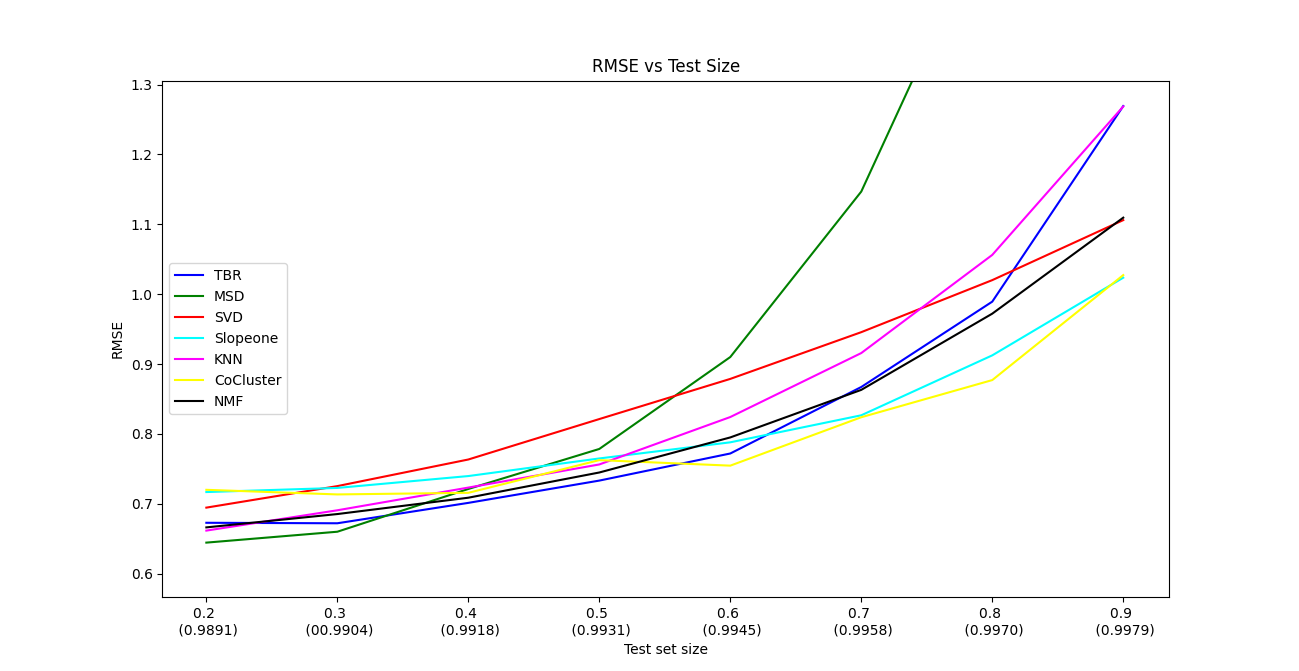
\includegraphics[scale=0.42]{rmse.png}
	\caption{RMSE versus Testset Size. For instance, 0.2 means testset-trainset ratio is $20\%-80\%$ . Additionally, floats in parentheses represent the sparsity of trainset for corresponding test set size}
	\label{fig:rmse}
\end{figure}

\begin{figure}[H]
	\centering
	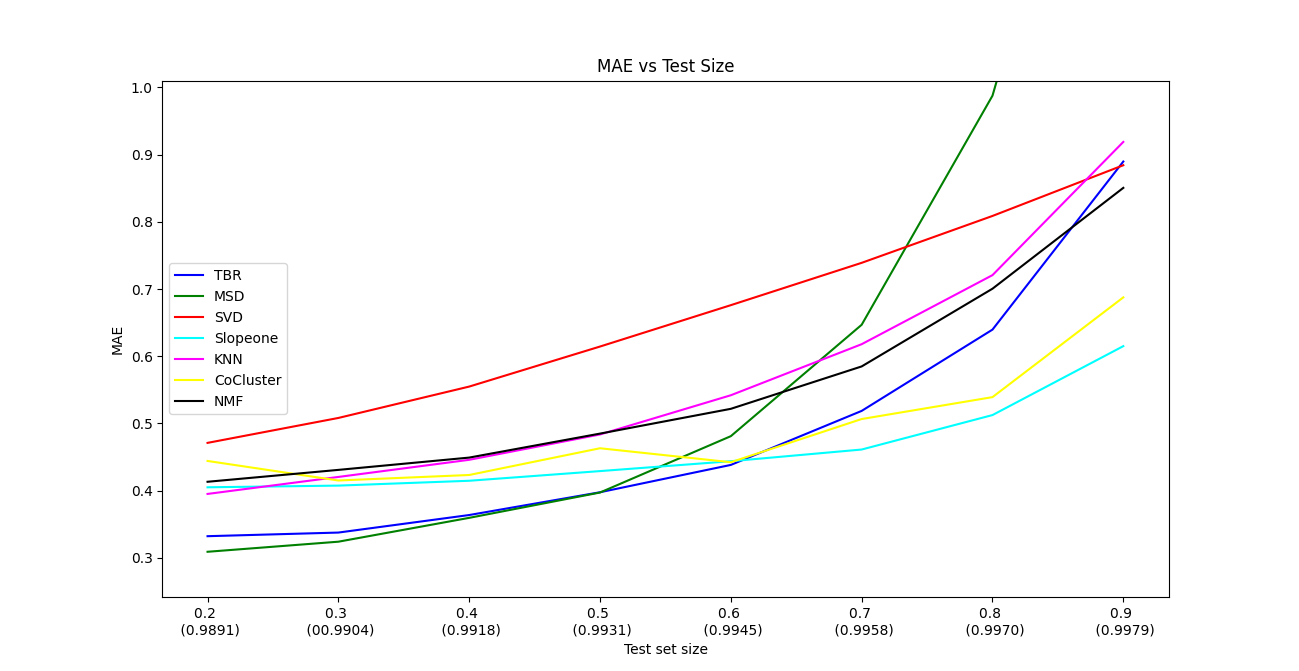
\includegraphics[scale=0.42]{mae.png}
	\caption{MAE versus Testset Size}
	\label{fig:mae}
\end{figure}
	
	\subsubsection{Libraries I Used}
	\paragraph{Surprise \cite{Surprise}} \mbox{} \\
	Surprise is a Python library for building and analyzing recommender systems. We use it for evaluating the performance of the trust based recommenders on various datasets and comparing them with the provided built-in recommender systems.
	\label{surprise}
	\subparagraph{Installation}:
	\begin{lstlisting}[language=bash]
	pip install scikit-surprise
	\end{lstlisting}
	
	\subparagraph{Sample Usage}:
	\begin{lstlisting}[language=python, caption=Surprise example]
	from surprise import AlgoBase, PredictionImpossible, Dataset
	from surprise.model_selection import cross_validate
	
	class Inverse_distance_weighted_tbr(AlgoBase):
	...
	
	reader = reader = Reader(line_format='user item rating timestamp', sep=';', rating_scale=(1, 5))
	
	data = Dataset.load_from_file('./dataset.csv', reader=reader)
	algo = Inverse_distance_weighted_tbr()
	
	cross_validate(algo, data, cv=5, verbose=True)
	\end{lstlisting}
	
	\paragraph{Matplotlib \cite{Matplotlib}} \mbox{} \\
	Matplotlib is a comprehensive library for creating static, animated, and interactive visualizations in Python. We use it to visualize the evaluation results of the recommenders and  statistical properties of the dataset such as the distribution of Eigentrust.
	\subparagraph{Installation}:
	\begin{lstlisting}[language=bash]
	pip install matplotlib
	\end{lstlisting}
	
	\subparagraph{Sample Usage}:
	\begin{lstlisting}[language=python, caption=Matplotlib example]
	import matplotlib.pyplot as plt
	...
	plt.hist(eigentrust_list, 
	color = 'blue', 
	edgecolor = 'black',
	bins = bins)
	plt.title('Distribution of the Eigentrust Values')
	plt.xlabel('Range')
	plt.ylabel('Number of Eigentrust Values in the range')
	plt.show() 
	\end{lstlisting}